\documentclass[12pt]{article}
\renewcommand{\baselinestretch}{0.95}

\usepackage{sbc-template}
\usepackage{graphicx,url}
\usepackage[utf8]{inputenc}
\makeatletter\let\normalsfcodes\relax\makeatother
\usepackage[brazil]{babel}
\AtBeginDocument{\providecommand{\normalsfcodes}{}}
\usepackage{booktabs}
\usepackage{tabularx}
\usepackage{tikz}
\usepackage{amsmath}
\usepackage{amssymb}
\usepackage{enumitem}
\usepackage[table]{xcolor}
\usepackage{multirow}
\usepackage{pgfgantt}
\usetikzlibrary{arrows.meta, positioning, shapes.geometric, fit, backgrounds, calc}
\makeatletter
\providecommand\normalsfcodes{%
  \sfcode`\.=\@m
  \sfcode`\?=\@m
  \sfcode`\!=\@m
  \sfcode`\:=\@m
  \sfcode`\;=\@m
}
\makeatother

\newcommand{\code}[1]{\texttt{#1}}
\newcommand{\proj}{AI-CogWalk}
\def\UrlBreaks{\do\/\do-}
\newcolumntype{Y}{>{\raggedright\arraybackslash}X}

\title{\proj: Detecção de Barreiras de Usabilidade para Usuários Iniciantes por meio de Agentes Multimodais e Evidências de Interação Humana}

\author{Lucas Matheus Silva\inst{1}}
\address{Instituto Federal da Paraíba (IFPB)\\Laboratório de Inovação em Software (LIS)}

\begin{document}
\maketitle
\sloppy

%%%%%%%%%%%%%%%%%%%%%%%%%%%%%%%%%%%%%%
\begin{abstract}
Multimodal agents built on large language models (LLMs) can now complete tasks in web interfaces, and recent work uses them to run cognitive walkthroughs and simulated usability tests. Completing a task, however, is not the same as noticing what makes it hard for a novice: in a recent comparison, LLM agents completed more tasks than human participants but anticipated only a fraction of the points where humans failed. This research proposal presents \textit{\proj}, an AI-assisted cognitive walkthrough that structures the diagnosis around the four classic walkthrough questions, reports each suspected barrier with its visual evidence, criterion and calibrated confidence, and uses human interaction evidence kept strictly separate from the data used to test it. The main comparison asks whether difficulty patterns observed in other applications improve the precision, coverage and calibration of alerts on web interfaces not used for calibration, against a strong baseline that already uses the navigation context. The reference is what novice participants actually experience; expert inspection is a comparison method, and the sample size will be set by a pilot study. The contribution sought is a validated method, a prototype and an annotated dataset; a negative result, showing where and why agents miss human difficulties, is also a planned outcome.
\end{abstract}

\begin{resumo}
Agentes multimodais baseados em modelos de linguagem de grande escala (LLMs) já conseguem concluir tarefas em interfaces web, e trabalhos recentes os usam para executar percursos cognitivos e testes de usabilidade simulados. Concluir a tarefa, porém, não é o mesmo que perceber o que a torna difícil para um usuário iniciante: numa comparação recente, agentes concluíram mais tarefas do que participantes humanos, mas anteciparam só uma fração dos pontos em que os humanos falharam. Este projeto de pesquisa apresenta o \textit{\proj}, um percurso cognitivo assistido por IA que organiza o diagnóstico nas quatro perguntas clássicas do método, registra cada suspeita de barreira com sua evidência visual, o critério violado e uma confiança calibrada, e usa evidências de interação humana mantidas estritamente separadas dos dados usados para avaliá-lo. A comparação principal investiga se padrões de dificuldade observados em outras aplicações melhoram a precisão, a cobertura e a calibração dos alertas em interfaces web não usadas na calibração, frente a uma \textit{baseline} forte que já usa o contexto da navegação. A referência é o que participantes iniciantes de fato experimentam; a inspeção por especialistas é um método comparativo, e o tamanho da amostra será definido por um estudo piloto. A contribuição buscada é um método validado experimentalmente, um protótipo e um conjunto de dados anotado; um resultado negativo, que mostre onde e por que os agentes deixam de perceber dificuldades humanas, também é um resultado previsto.
\end{resumo}

%%%%%%%%%%%%%%%%%%%%%%%%%%%%%%%%%%%%%%
\section{Introdução}
\label{sec:intro}

Avaliar a usabilidade de uma interface com usuários reais é caro: exige recrutar participantes, conduzir sessões, analisar gravações e consolidar problemas. Por isso, métodos de inspeção, em que especialistas examinam a interface sem usuários, são usados há décadas. O \textit{percurso cognitivo} (\textit{cognitive walkthrough}) é um deles e foi criado justamente para avaliar a facilidade de aprendizagem por exploração, isto é, se uma pessoa que nunca usou o sistema consegue descobrir, passo a passo, como realizar uma tarefa \cite{polson1992cw,wharton1994cw}.

Agentes multimodais baseados em LLMs mudaram o custo dessa inspeção. Eles leem capturas de tela e a estrutura da página e executam tarefas em \textit{sites} reais \cite{deng2023mind2web,zhou2024webarena}. Trabalhos recentes já os usam para conduzir percursos cognitivos \cite{bisante2024cwgpt,zhong2025syntheticcw}, avaliações heurísticas \cite{zhong2025syntheticheuristic,guerino2025gpt4o,duan2024mockups} e testes com usuários simulados por \textit{personas} \cite{lu2025uxagent,tan2026avenirux,holter2026uxcascade,bougie2026perceptui}.

O problema é que um agente bom em \textit{concluir} uma tarefa não é, por isso, bom em \textit{perceber} onde ela é difícil. No estudo do \textit{Synthetic Cognitive Walkthrough} \cite{zhong2025syntheticcw}, os agentes concluíram as tarefas com mais frequência do que os participantes humanos, mas os pontos de falha que eles anteciparam foram poucos perto dos que os humanos de fato encontraram. Um agente que escolhe a opção mais provável de um menu ambíguo e segue em frente cumpre a tarefa e esconde exatamente a dificuldade que um iniciante teria. Se ferramentas desse tipo passarem a ser usadas no lugar de parte dos testes com pessoas, alertas faltantes, ou alertas inventados, viram decisões de projeto erradas.

Este projeto propõe o \textit{\proj}, um percurso cognitivo assistido por agentes multimodais que (i) estrutura o diagnóstico nas quatro perguntas do método, por etapa da tarefa; (ii) registra cada suspeita como um alerta rastreável, separando fato observado, hipótese sobre o comportamento humano e recomendação; e (iii) incorpora evidências de interação humana de forma controlada, sem que o sistema veja as respostas dos participantes usados para avaliá-lo. A pergunta central é: \textit{em que medida a incorporação de padrões de dificuldades observadas em usuários reais melhora a precisão, a cobertura e a confiabilidade dos alertas gerados por agentes multimodais durante percursos cognitivos de interfaces web não utilizadas na calibração?} A generalização para interfaces novas fica, assim, no centro da investigação.

As contribuições pretendidas são: (i) uma caracterização empírica dos tipos de dificuldade de usuários iniciantes que agentes multimodais identificam ou deixam passar; (ii) o método \proj, com o formato de alerta e o protocolo de separação entre dados de calibração e de teste; (iii) um protótipo; e (iv) um conjunto de dados anotado, com tarefas, telas, rastros de interação anonimizados e problemas confirmados por avaliadores independentes. A originalidade não está em usar um LLM para avaliar usabilidade, o que já foi feito, nem em usar exemplos humanos para alinhar agentes sintéticos, o que o PerceptUI \cite{bougie2026perceptui} já faz para preferências e julgamentos de interface, mas em identificar \textit{barreiras cognitivas localizadas em etapas de tarefas} e em medir a validade desses alertas contra dificuldades observadas em iniciantes, em interfaces não usadas na calibração.

\textbf{Relação com os temas.}
O projeto se insere no Tema 8, \textit{Aplicação de Técnicas Inteligentes na Solução de Problemas em Engenharia de Software}: a avaliação de usabilidade é uma atividade de qualidade de software, e o projeto aplica agentes multimodais a um problema dela, a detecção de barreiras para iniciantes, medindo quando a técnica funciona e quando falha. A relação com o Tema 7 é indireta e dependeria de integrar a ferramenta a processos de validação de software, por exemplo em ambientes de homologação, como etapa de inspeção antes dos testes com usuários.

O texto está organizado assim: a Seção~\ref{sec:problema} ilustra o problema; a Seção~\ref{sec:fundamentacao} apresenta a fundamentação; a Seção~\ref{sec:relacionados} discute trabalhos relacionados e a lacuna; a Seção~\ref{sec:abordagem} descreve a abordagem; a Seção~\ref{sec:experimento} detalha o desenho experimental; a Seção~\ref{sec:etica} trata dos aspectos éticos; a Seção~\ref{sec:plano} apresenta o plano de pesquisa; a Seção~\ref{sec:ameacas} discute ameaças à validade; e a Seção~\ref{sec:final} conclui.

%%%%%%%%%%%%%%%%%%%%%%%%%%%%%%%%%%%%%%
\section{O Problema: Concluir a Tarefa não é Perceber a Dificuldade}
\label{sec:problema}

Considere um portal acadêmico em que o estudante precisa emitir uma declaração de matrícula (Figura~\ref{fig:portal}; a interface é fictícia e serve só para ilustrar a hipótese). A tela inicial oferece quatro opções: \textit{Acadêmico}, \textit{Documentos}, \textit{Protocolos} e \textit{Serviços}. Um estudante iniciante pode associar a declaração a três delas e não saber qual escolher.

\begin{figure}[!ht]
\centering
\begin{tikzpicture}[
  font=\small,
  btn/.style={draw=blue!50, fill=blue!6, rounded corners=2pt, minimum width=2.4cm, minimum height=0.75cm},
  amb/.style={btn, draw=orange!80!black, fill=orange!10, line width=0.8pt}]
  \node[draw=gray!60, fill=gray!8, minimum width=11.6cm, minimum height=0.6cm, anchor=west] (bar) at (0,0) {\textbf{Portal do Estudante}};
  \node[anchor=west] (q) at (0.2,-0.8) {O que você deseja acessar?};
  \node[amb, anchor=west] (a) at (0.2,-1.7) {Acadêmico};
  \node[amb, right=0.4cm of a] (d) {Documentos};
  \node[btn, right=0.4cm of d] (p) {Protocolos};
  \node[amb, right=0.4cm of p] (s) {Serviços};
  \node[draw=gray!60, fit=(bar)(q)(a)(s), inner sep=4pt] {};
  \node[anchor=north west, align=left, font=\scriptsize, text width=11.4cm] at (0.1,-2.4)
   {Tarefa: \textit{obter uma declaração de matrícula}. Em laranja, as opções que um iniciante pode associar ao objetivo.};
\end{tikzpicture}
\caption{Interface fictícia usada como exemplo.}
\label{fig:portal}
\end{figure}

Um agente orientado à conclusão escolhe a opção mais provável, digamos \textit{Documentos}, e segue até encontrar a declaração; se errar, volta e tenta outra. Ao final, reporta sucesso. O que o \proj\ deveria fazer é diferente: perceber que mais de uma opção representa a intenção do estudante, registrar essa ambiguidade como possível barreira de aprendizagem e marcá-la como \textit{suspeita}, a ser confirmada ou descartada por evidência humana. A Tabela~\ref{tab:registro} mostra o registro que o sistema produziria.

\begin{table}[!ht]
\centering
\caption{Registro ilustrativo de um alerta do \proj\ para o exemplo da Figura~\ref{fig:portal}.}
\label{tab:registro}
\small
\begin{tabularx}{0.92\linewidth}{@{}l Y l@{}}
\toprule
\textbf{Campo} & \textbf{Conteúdo} & \textbf{Natureza} \\
\midrule
Tarefa & Emitir declaração de matrícula & contexto \\
Etapa & Seleção da seção inicial & contexto \\
Critério & Q3: o usuário associa a ação ao seu objetivo? & teoria \\
Evidência visual & Três rótulos semanticamente próximos do objetivo, sem texto de apoio & fato observado \\
Diagnóstico & Rótulos potencialmente ambíguos para a tarefa & hipótese \\
Evidência humana & Na calibração, iniciantes divergiram entre caminhos em telas com rótulos análogos & evidência \\
Estado & Suspeita pendente de validação & --- \\
Confiança & Calibrada a partir do histórico de acertos do sistema (Seção~\ref{sec:abordagem}) & --- \\
Recomendação & Testar rótulos mais explícitos ou um atalho para ``Declarações'' & recomendação \\
\bottomrule
\end{tabularx}
\end{table}

A coluna ``Natureza'' é parte da proposta. A presença de várias opções semelhantes, por si só, não comprova um defeito: pode ser que todos os caminhos levem à declaração, ou que os estudantes já conheçam o portal. O alerta precisa deixar claro o que foi observado na tela, o que é suposição sobre pessoas e o que é sugestão de mudança, para que o avaliador humano decida o que fazer.

%%%%%%%%%%%%%%%%%%%%%%%%%%%%%%%%%%%%%%
\section{Fundamentação}
\label{sec:fundamentacao}

\textbf{Percurso cognitivo.} O método parte de uma tarefa, de um perfil de usuário e da sequência correta de ações. Para cada ação, o avaliador responde a quatro perguntas \cite{wharton1994cw}: \textbf{Q1}, o usuário tentará atingir o efeito correto (tem o objetivo certo naquele momento)? \textbf{Q2}, perceberá que a ação correta está disponível? \textbf{Q3}, associará a ação ao efeito que deseja? \textbf{Q4}, se a ação for executada, perceberá que progrediu? Cada resposta negativa, com sua justificativa, é uma ``história de falha''. Versões simplificadas reduzem as perguntas para tornar o método viável em equipes de desenvolvimento \cite{spencer2000streamlined}. No \proj, as quatro perguntas são a estrutura do diagnóstico: cada alerta precisa apontar qual delas falha, em qual etapa e com qual evidência.

\textbf{Avaliar um método de avaliação.} A literatura de avaliação de métodos define \cite{hartson2003criteria} as medidas usadas para comparar métodos de avaliação de usabilidade: \textit{completude} (\textit{thoroughness}), a fração dos problemas reais encontrada pelo método, e \textit{validade}, a fração dos problemas apontados que são reais. Elas correspondem a \textit{recall} e precisão, e dependem de um conjunto de referência de problemas reais, normalmente obtido em testes com usuários. Também se sabe que avaliadores humanos diferentes encontram conjuntos de problemas bem diferentes na mesma interface, o chamado efeito do avaliador \cite{hertzum2001evaluator}, e que o número de problemas encontrados cresce com o número de avaliadores ou participantes \cite{nielsen1993model}. Isso tem duas consequências para este projeto: a referência humana precisa ser construída com mais de um avaliador e com concordância medida \cite{cohen1960kappa}, e a comparação justa do agente é com um especialista, não com uma lista ``completa'' de problemas que nenhum método atinge.

\textbf{Agentes multimodais em interfaces.} Agentes que recebem a captura de tela e a árvore de elementos e escolhem a próxima ação foram desenvolvidos para \textit{concluir} tarefas, e são avaliados por taxa de sucesso \cite{deng2023mind2web,zhou2024webarena}. Usá-los para avaliar usabilidade inverte o objetivo: o que interessa não é o sucesso do agente, mas as hesitações, enganos e pedidos de ajuda que um humano teria no mesmo caminho.

%%%%%%%%%%%%%%%%%%%%%%%%%%%%%%%%%%%%%%
\section{Trabalhos Relacionados e Lacuna}
\label{sec:relacionados}

A Tabela~\ref{tab:relacionados} resume os trabalhos mais próximos, organizados pelo que cada um faz e pelo que deixa em aberto para esta pesquisa. A leitura foi feita a partir dos textos disponíveis em novembro de 2026 e será aprofundada na revisão sistemática (Seção~\ref{sec:plano}).

\begin{table}[!ht]
\centering
\caption{Trabalhos mais próximos ao \proj.}
\label{tab:relacionados}
\footnotesize
\begin{tabularx}{\linewidth}{@{}>{\raggedright\arraybackslash}p{2.6cm} Y Y@{}}
\toprule
\textbf{Trabalho} & \textbf{O que faz} & \textbf{O que deixa em aberto} \\
\midrule
CWGPT \cite{bisante2024cwgpt} & Agente conversacional sobre GPT-4 que conduz avaliações inspiradas no percurso cognitivo em aplicações web; estudo exploratório com aplicações de estudantes. & Avaliação exploratória, sem medir precisão e \textit{recall} contra problemas observados em usuários. \\
\addlinespace
\textit{Synthetic Cognitive Walkthrough} \cite{zhong2025syntheticcw} & Agentes (GPT-4 e Gemini 2.5 Pro) executam percursos cognitivos em dois aplicativos móveis e são comparados com 10 participantes; agentes concluem mais tarefas e antecipam poucos dos pontos de falha humanos; o contexto da navegação melhora a previsão. & Duas interfaces; não usa evidências humanas para melhorar o agente; é a \textit{baseline} forte (C2) deste projeto. \\
\addlinespace
Avaliação heurística por LLM \cite{zhong2025syntheticheuristic,guerino2025gpt4o,duan2024mockups} & Compara problemas apontados por LLMs com os de especialistas em avaliação heurística. & Foco em heurísticas gerais, não em aprendizagem por exploração de iniciantes. \\
\addlinespace
UXAgent, Avenir-UX \cite{lu2025uxagent,tan2026avenirux} & Agentes com \textit{personas} navegam em \textit{sites}, registram etapas e geram relatórios; o Avenir-UX inclui pensamento em voz alta e SEQ/SUS simulados, com código aberto (Playwright). & Não há evidência publicada de que alertas e pontuações correspondam a problemas observados em usuários; Avenir-UX é candidato a \textit{baseline} e infraestrutura. \\
\addlinespace
UXCascade \cite{holter2026uxcascade} & Ferramenta para profissionais de UX analisarem execuções de agentes simulados; estudo com 8 profissionais e problemas semeados. & Problemas semeados pelos autores, não observados em usuários reais. \\
\addlinespace
PerceptUI \cite{bougie2026perceptui} & Usa respostas humanas para treinar agentes de \textit{persona} cujas preferências e avaliações de interfaces se alinham às de usuários. & É o mais próximo do uso de evidência humana; mas alinha julgamentos sobre a interface, não localiza barreiras cognitivas por etapa de tarefa. \\
\addlinespace
GUIDE \cite{yang2026guide} & \textit{Benchmark} com 120 demonstrações de iniciantes (67,5 h, pensamento em voz alta) em 10 programas complexos; detecção de estado, intenção e necessidade de ajuda. & Rótulos de comportamento, não problemas de percurso cognitivo; exige mapeamento metodológico. \\
\addlinespace
Rico \cite{deka2017rico} & Telas, hierarquias de componentes, anotações semânticas e rastros de interação de milhares de aplicativos Android. & Não contém referência validada de dificuldades de iniciantes. \\
\bottomrule
\end{tabularx}
\end{table}

\textbf{Lacuna.} Simular \textit{personas}, navegar e gerar relatórios de usabilidade já não basta para reivindicar originalidade. Também não se pode atribuir a um método novo um ganho que já vem do uso do contexto da navegação, mostrado no \textit{Synthetic Cognitive Walkthrough} \cite{zhong2025syntheticcw}. O que os trabalhos acima ainda não oferecem, em conjunto, é: (i) alertas estruturados por pergunta do percurso cognitivo e por etapa, com evidência e estado explícitos; (ii) uso de padrões de dificuldade observados em pessoas para melhorar o agente na \textit{localização} dessas barreiras, com separação rigorosa entre dados de calibração e de teste (o PerceptUI usa dados humanos, mas para alinhar preferências e avaliações globais); e (iii) avaliação da validade desses alertas contra problemas observados em iniciantes reais, em interfaces não vistas, com análise de estabilidade e custo. A originalidade definitiva dependerá de comparar o \proj\ com CWGPT, \textit{Synthetic Cognitive Walkthrough} e Avenir-UX, e com o PerceptUI, sob o mesmo protocolo, e de mostrar um ganho que essas abordagens não entregam, ou de explicar por que ele não aparece.

%%%%%%%%%%%%%%%%%%%%%%%%%%%%%%%%%%%%%%
\section{Abordagem Proposta}
\label{sec:abordagem}

O \proj\ não treina um modelo novo. Ele organiza o trabalho de um modelo multimodal existente em um fluxo controlado, em quatro estágios: \textit{configurar} a tarefa, \textit{navegar} pelo caminho correto capturando cada tela, \textit{avaliar} cada etapa com as quatro perguntas do percurso cognitivo e \textit{revisar} os alertas, com registro de tudo o que foi enviado ao modelo e do que ele respondeu. A Figura~\ref{fig:arquitetura} mostra os componentes; o restante desta seção descreve cada estágio.

\begin{figure}[!ht]
\centering
\resizebox{\linewidth}{!}{%
\begin{tikzpicture}[
  font=\small,
  mod/.style={draw=violet!70, fill=violet!6, rounded corners=2pt, align=center, minimum height=1.15cm, text width=2.45cm, font=\footnotesize},
  ext/.style={draw=gray!70, fill=gray!8, rounded corners=3pt, align=center, minimum height=1.0cm, text width=2.45cm, font=\footnotesize},
  ui/.style={draw=blue!60, fill=blue!6, rounded corners=3pt, align=center, minimum height=1.0cm, text width=2.45cm, font=\footnotesize},
  hum/.style={draw=green!50!black, fill=green!8, rounded corners=3pt, align=center, minimum height=1.0cm, text width=2.45cm, font=\footnotesize},
  arr/.style={-{Stealth[length=2mm]}, gray!70!black, line width=0.7pt},
  darr/.style={arr, dashed}]
  % linha superior: pessoas e fontes externas
  \node[hum] (rev)  at (0,0)  {\textbf{Pesquisador e revisor}};
  \node[ui]  (ui)   at (3,0)  {\textbf{Painel web}\\ tarefas, telas, revisão};
  \node[ext] (site) at (6,0)  {\textbf{Site avaliado}\\ só leitura (GET)};
  \node[hum] (ex)   at (9,0)  {\textbf{Padrões humanos}\\ de \textit{outras} aplicações};
  % servidor
  \node[mod] (cad)  at (0,-2.1) {\textbf{Cadastro}\\ projeto, \textit{hosts}, tarefa};
  \node[mod] (orq)  at (3,-2.1) {\textbf{Orquestração}\\ fila, condição C1--C3};
  \node[mod] (nav)  at (6,-2.1) {\textbf{Navegação}\\ capturas e elementos};
  \node[mod] (ava)  at (9,-2.1) {\textbf{Avaliação Q1--Q4}\\ \textit{prompt} versionado};
  \node[mod] (rel)  at (3,-3.75) {\textbf{Relatórios}\\ HTML, MD, JSON, ZIP};
  \node[mod] (reg)  at (6,-3.75) {\textbf{Registro}\\ \textit{prompt}, \textit{hash}, resposta, custo};
  \node[mod] (ver)  at (9,-3.75) {\textbf{Verificação (C3)}\\ elementos + verificador};
  \begin{scope}[on background layer]
    \node[draw=violet!50, rounded corners=4pt, fit=(cad)(ava)(ver)(rel), inner sep=7pt] (srv) {};
  \end{scope}
  \node[font=\footnotesize\bfseries, violet!70!black, anchor=south west] at (srv.south west) {Servidor};
  % externos à direita e abaixo
  \node[ext] (llm) at (12.2,-2.95) {\textbf{Modelo multimodal}\\ (API) ou avaliador \textit{offline}};
  \node[ext] (db)  at (1.5,-6.0) {\textbf{Banco relacional}\\ execuções, alertas, revisões};
  \node[ext] (fs)  at (4.5,-6.0) {\textbf{Armazenamento}\\ telas, HTML, \textit{cache}};
  % ligações
  \draw[arr] (rev) -- (ui);
  \draw[arr] (ui) -- node[right, font=\scriptsize]{API} (orq);
  \draw[arr] (cad) -- (orq); \draw[arr] (orq) -- (nav); \draw[arr] (nav) -- (ava);
  \draw[arr, <->] (nav) -- (site);
  \draw[darr] (ex) -- node[right, font=\scriptsize]{C3a} (ava);
  \draw[arr] (ava) -- (ver);
  \draw[arr] (ava) -- (reg); \draw[arr] (ver) -- (reg); \draw[arr] (reg) -- (rel);
  \draw[arr, <->] (ava.east) -- (llm.north west);
  \draw[arr, <->] (ver.east) -- (llm.south west);
  \draw[arr] (srv.south -| db) -- (db);
  \draw[arr] (srv.south -| fs) -- (fs);
\end{tikzpicture}}
\caption{Arquitetura do \proj, como implementada no protótipo. O servidor só acessa o site avaliado com requisições de leitura, e as evidências humanas (linha tracejada) vêm de aplicações diferentes da avaliada.}
\label{fig:arquitetura}
\end{figure}

\subsection{Configuração da tarefa}

O pesquisador cadastra o \textit{projeto} (o sistema avaliado, sua URL e a lista de \textit{hosts} autorizados) e a \textit{tarefa}: o objetivo em linguagem natural, o perfil do usuário (por exemplo, ``estudante que nunca acessou a área de editais''), o conhecimento esperado e a \textit{sequência correta de ações}. Cada ação é \textit{clicar} em um elemento ou \textit{localizar} um item na tela, identificado pelo rótulo visível. Fornecer o caminho correto é a premissa do percurso cognitivo \cite{wharton1994cw}: o método não pergunta se o agente consegue concluir a tarefa, mas se um iniciante perceberia, em cada etapa, a ação que leva ao objetivo.

\subsection{Navegação controlada}

Um navegador automatizado percorre o caminho correto e, antes de cada ação, captura a tela visível, a página inteira, o HTML e a lista de elementos interativos com rótulo, tipo, destino, posição e se estão visíveis sem rolar. Cada elemento recebe um identificador (\code{e1}, \code{e2}, \ldots), que o modelo deve usar ao citar evidências. Ao final, captura-se também a tela alcançada. A navegação segue uma política de segurança: só acessa os \textit{hosts} autorizados, só faz requisições de leitura (GET), nunca clica em elementos dentro de formulários, não aceita \textit{downloads} e espera um intervalo configurável entre as ações. Se um rótulo da tarefa não é encontrado ou a página sai do domínio autorizado, a execução para e guarda as telas já capturadas, para que a falha possa ser inspecionada.

\subsection{Avaliação por etapa}

Para cada ação, o modelo recebe a tela em que ela precisa ser executada (imagem e lista de elementos), a tela resultante (para Q4) e, conforme a condição, o histórico das telas e ações anteriores. Ele responde Q1 a Q4 separadamente, cada uma com \textit{sim}, \textit{não} ou \textit{incerto} e uma justificativa, em JSON com esquema fixo. Só uma resposta \textit{não} gera alerta. A Tabela~\ref{tab:entradas} resume o que cada condição recebe; a estratégia de \textit{prompting} é discutida na Seção~\ref{sec:experimento}.

\begin{table}[!ht]
\centering
\caption{O que o modelo recebe em cada condição.}
\label{tab:entradas}
\footnotesize
\begin{tabularx}{\linewidth}{@{}l c c c Y@{}}
\toprule
\textbf{Condição} & \textbf{Tela + elementos} & \textbf{Histórico} & \textbf{Verificação} & \textbf{Evidência humana} \\
\midrule
C1 & \checkmark & -- & -- & -- \\
C2 & \checkmark & \checkmark & -- & -- \\
C3a & \checkmark & \checkmark & \checkmark & padrões de outras aplicações \\
C3b & \checkmark & \checkmark & \checkmark & C3a + rastros de poucos participantes extras da mesma aplicação \\
\bottomrule
\end{tabularx}
\end{table}

Cada alerta separa três coisas: a \textit{evidência visual}, que descreve só o que está na tela e cita os identificadores dos elementos; o \textit{diagnóstico}, que é a hipótese sobre a dificuldade do iniciante; e a \textit{recomendação}, que é uma mudança a testar. Essa separação permite verificar o fato sem precisar concordar com a hipótese.

\subsection{Verificação de evidências}

Na condição C3, cada alerta passa por dois testes antes de chegar ao revisor. O primeiro é determinístico: os elementos citados precisam existir na captura. O segundo é uma chamada independente ao modelo, que vê só a tela, a lista de elementos e o alerta, e responde se a evidência descrita existe e se ela torna plausível uma dificuldade real ou é apenas um fato neutro. Um alerta que falha em qualquer teste é rebaixado para \textit{não confirmado}, em vez de ser descartado em silêncio, e a justificativa fica registrada.

\subsection{Evidências humanas e dois protocolos}

As evidências humanas são rastros de interação (cliques, retornos, tempo parado, pedidos de ajuda e falas em voz alta), já interpretados por avaliadores. Delas se extraem padrões de dificuldade com exemplos, como ``em telas com opções de nomes próximos, iniciantes divergiram entre caminhos'', que entram no contexto do modelo como casos de referência. O sistema nunca recebe os rastros dos participantes cujas sessões formam a referência de teste, e cada execução registra quais casos recebeu. Há dois protocolos, com hipóteses e resultados próprios:
\begin{itemize}[noitemsep, topsep=3pt, leftmargin=1.5em]
  \item \textbf{Protocolo G (generalização), condição C3a:} os padrões vêm só de \textit{outras} aplicações, as de calibração. Responde se o conhecimento sobre dificuldades humanas transfere para interfaces nunca vistas. É o protocolo principal da dissertação.
  \item \textbf{Protocolo A (adaptação), condição C3b:} além dos padrões de C3a, o sistema recebe rastros de poucos participantes adicionais (por exemplo, dois) na \textit{mesma} aplicação. Não é uma avaliação em aplicação desconhecida, e seus resultados são reportados à parte.
\end{itemize}

\subsection{Calibração da confiança}

O modelo declara uma confiança para cada alerta, mas essa declaração, sozinha, não é confiável. A confiança reportada será estimada a partir da taxa de confirmação de alertas da mesma categoria nas aplicações de calibração, com encolhimento para a taxa global quando a categoria tem poucos exemplos, para que ``80\% de confiança'' signifique cerca de 80\% de alertas confirmados (métricas na Seção~\ref{sec:experimento}). Esse componente depende dos dados humanos e ainda não está implementado.

\subsection{Revisão, relatório e reprodutibilidade}

No painel, o revisor vê cada tela com o elemento-alvo e os elementos citados destacados, as respostas a Q1--Q4 e os alertas, e decide se cada um é \textit{procedente}, \textit{improcedente} ou \textit{inconclusivo}; o tempo gasto em cada decisão é registrado, porque ele compõe o custo do método. O relatório lista os alertas por tarefa e etapa com os campos da Tabela~\ref{tab:registro} e o estado de cada um: \textit{suspeita}, \textit{apoiada} (compatível com padrões da calibração) ou \textit{não confirmada}.

A reprodutibilidade é tratada desde o início. Cada execução guarda uma fotografia da configuração (condição, estratégia de \textit{prompt}, modelo, nível de esforço, versão do \textit{prompt}, tarefa e parâmetros do navegador). Cada chamada ao modelo guarda o texto enviado, um \textit{hash} das entradas, a resposta bruta, os \textit{tokens} e o tempo. Uma execução pode ser \textit{reavaliada} sobre as mesmas capturas, sem nova navegação, o que permite medir a variação entre repetições do modelo separada da variação do site. Um \textit{cache} de respostas, indexado pelo \textit{hash}, permite reproduzir uma avaliação idêntica. O pacote exportado reúne relatório, configuração, telas, HTML, \textit{prompts} e respostas de cada etapa.

%%%%%%%%%%%%%%%%%%%%%%%%%%%%%%%%%%%%%%
\section{Protótipo e Verificação Inicial}
\label{sec:prototipo}

Um protótipo do \proj\ já foi implementado para o Marco~1 do projeto, cujo critério de conclusão é \textit{reproduzir a mesma avaliação, visualizar as telas analisadas e exportar um relatório sem depender da leitura manual de registros}. O painel é uma aplicação web em Next.js; o servidor, em Java 21 com Spring Boot; os dados ficam em PostgreSQL; a navegação usa Playwright com Chromium; e a avaliação usa a API de um modelo multimodal ou, para testes sem custo, um \textit{avaliador offline} baseado em regras simples. Os componentes são empacotados em contêineres e podem ser publicados em uma plataforma de nuvem.

\textbf{Ambiente de teste controlado.} Para testar o fluxo sem depender de um site real, o protótipo inclui um portal fictício, servido pelo próprio servidor, que reproduz a estrutura do caso previsto para o piloto, o portal do Polo de Inovação do IFPB: a tarefa é localizar o ``Edital nº 01/2026 do Banco de Especialistas'' de um núcleo de inovação. O portal tem duas armadilhas inseridas de propósito: (i) na página do núcleo, o link correto chama-se apenas ``Editais'', enquanto um link vizinho, ``Banco de Especialistas'', repete os termos do objetivo, mas leva a uma página que lista os credenciamentos só até 2025; e (ii) na página de editais, o link ``Editais de 2026'' fica num arquivo por ano abaixo da área visível, depois de uma lista de editais recentes que não inclui o edital procurado.

\textbf{O que foi verificado.} A Tabela~\ref{tab:verificacao} resume as verificações executadas. Todas são \textit{verificações de funcionamento}: mostram que o fluxo navega, avalia, registra, reproduz e exporta como especificado. Elas não medem a qualidade dos alertas, que é a questão de pesquisa e depende de dados humanos.

\begin{table}[!ht]
\centering
\caption{Verificações executadas no protótipo (13/11/2026).}
\label{tab:verificacao}
\footnotesize
\begin{tabularx}{\linewidth}{@{}>{\raggedright\arraybackslash}p{3.6cm} Y >{\raggedright\arraybackslash}p{2.0cm}@{}}
\toprule
\textbf{Verificação} & \textbf{Como foi feita e o que se observou} & \textbf{Resultado} \\
\midrule
Política de navegação & Testes automatizados: aceita o domínio e subdomínios autorizados; recusa domínio parecido (\code{ifpb.edu.br.evil.com}), URL \code{javascript:}, método POST e elementos dentro de formulários & 5 testes de unidade passaram \\
Percurso completo (C3) & Teste de ponta a ponta no portal fictício: 4 ações, 5 telas capturadas, alvo encontrado em todas as etapas, Q1--Q4 respondidas nas 4 etapas, alertas com nota de verificação & Passou \\
Reprodução & Reavaliação das mesmas capturas: \textit{hash} das entradas e respostas idênticos aos da execução original, mesmo número de alertas & Passou \\
Estratégias de \textit{prompt} & Reavaliação com \textit{few-shot}: execução registra a versão do banco e os casos usados; o relatório avisa que o banco atual é ilustrativo & Passou \\
Revisão e exportação & Decisão do revisor registrada com tempo; relatório HTML com telas embutidas, Markdown, JSON e ZIP com telas, \textit{prompts} e respostas de cada etapa & Passou \\
Falha de navegação & Rótulo inexistente: execução marcada como falha, com mensagem clara e a tela já capturada preservada & Passou \\
Segurança do armazenamento & Pedido de arquivo fora do diretório de capturas (\code{../}) é recusado & Passou \\
Execução em contêineres & PostgreSQL, servidor com navegador e painel em contêineres separados, como na publicação em nuvem: 5 telas, 2 alertas, pacote de 1,1~MB & Passou \\
Portal real (piloto) & O ambiente de desenvolvimento não tem acesso ao domínio do portal; a execução falhou com erro de resolução de nome, reportado de forma legível & Pendente \\
\bottomrule
\end{tabularx}
\end{table}

\textbf{Exemplo de saída.} No portal fictício, com o avaliador \textit{offline} e a condição C3, o percurso levou cerca de 6~s (com 0,3~s de espera entre ações) e produziu dois alertas, um em cada armadilha: na etapa 2, Q3 (o rótulo ``Editais'' não tem os termos do objetivo, enquanto ``Banco de Especialistas'' tem); na etapa 3, Q2 (``Editais de 2026'' fica abaixo da área visível). A Figura~\ref{fig:mvp} mostra a tela de revisão da etapa 2. Esse resultado era esperado, porque as regras do avaliador \textit{offline} foram escritas para detectar exatamente esses dois padrões; ele serve para mostrar que o fluxo funciona de ponta a ponta, não que o método funciona.

\begin{figure}[!ht]
\centering
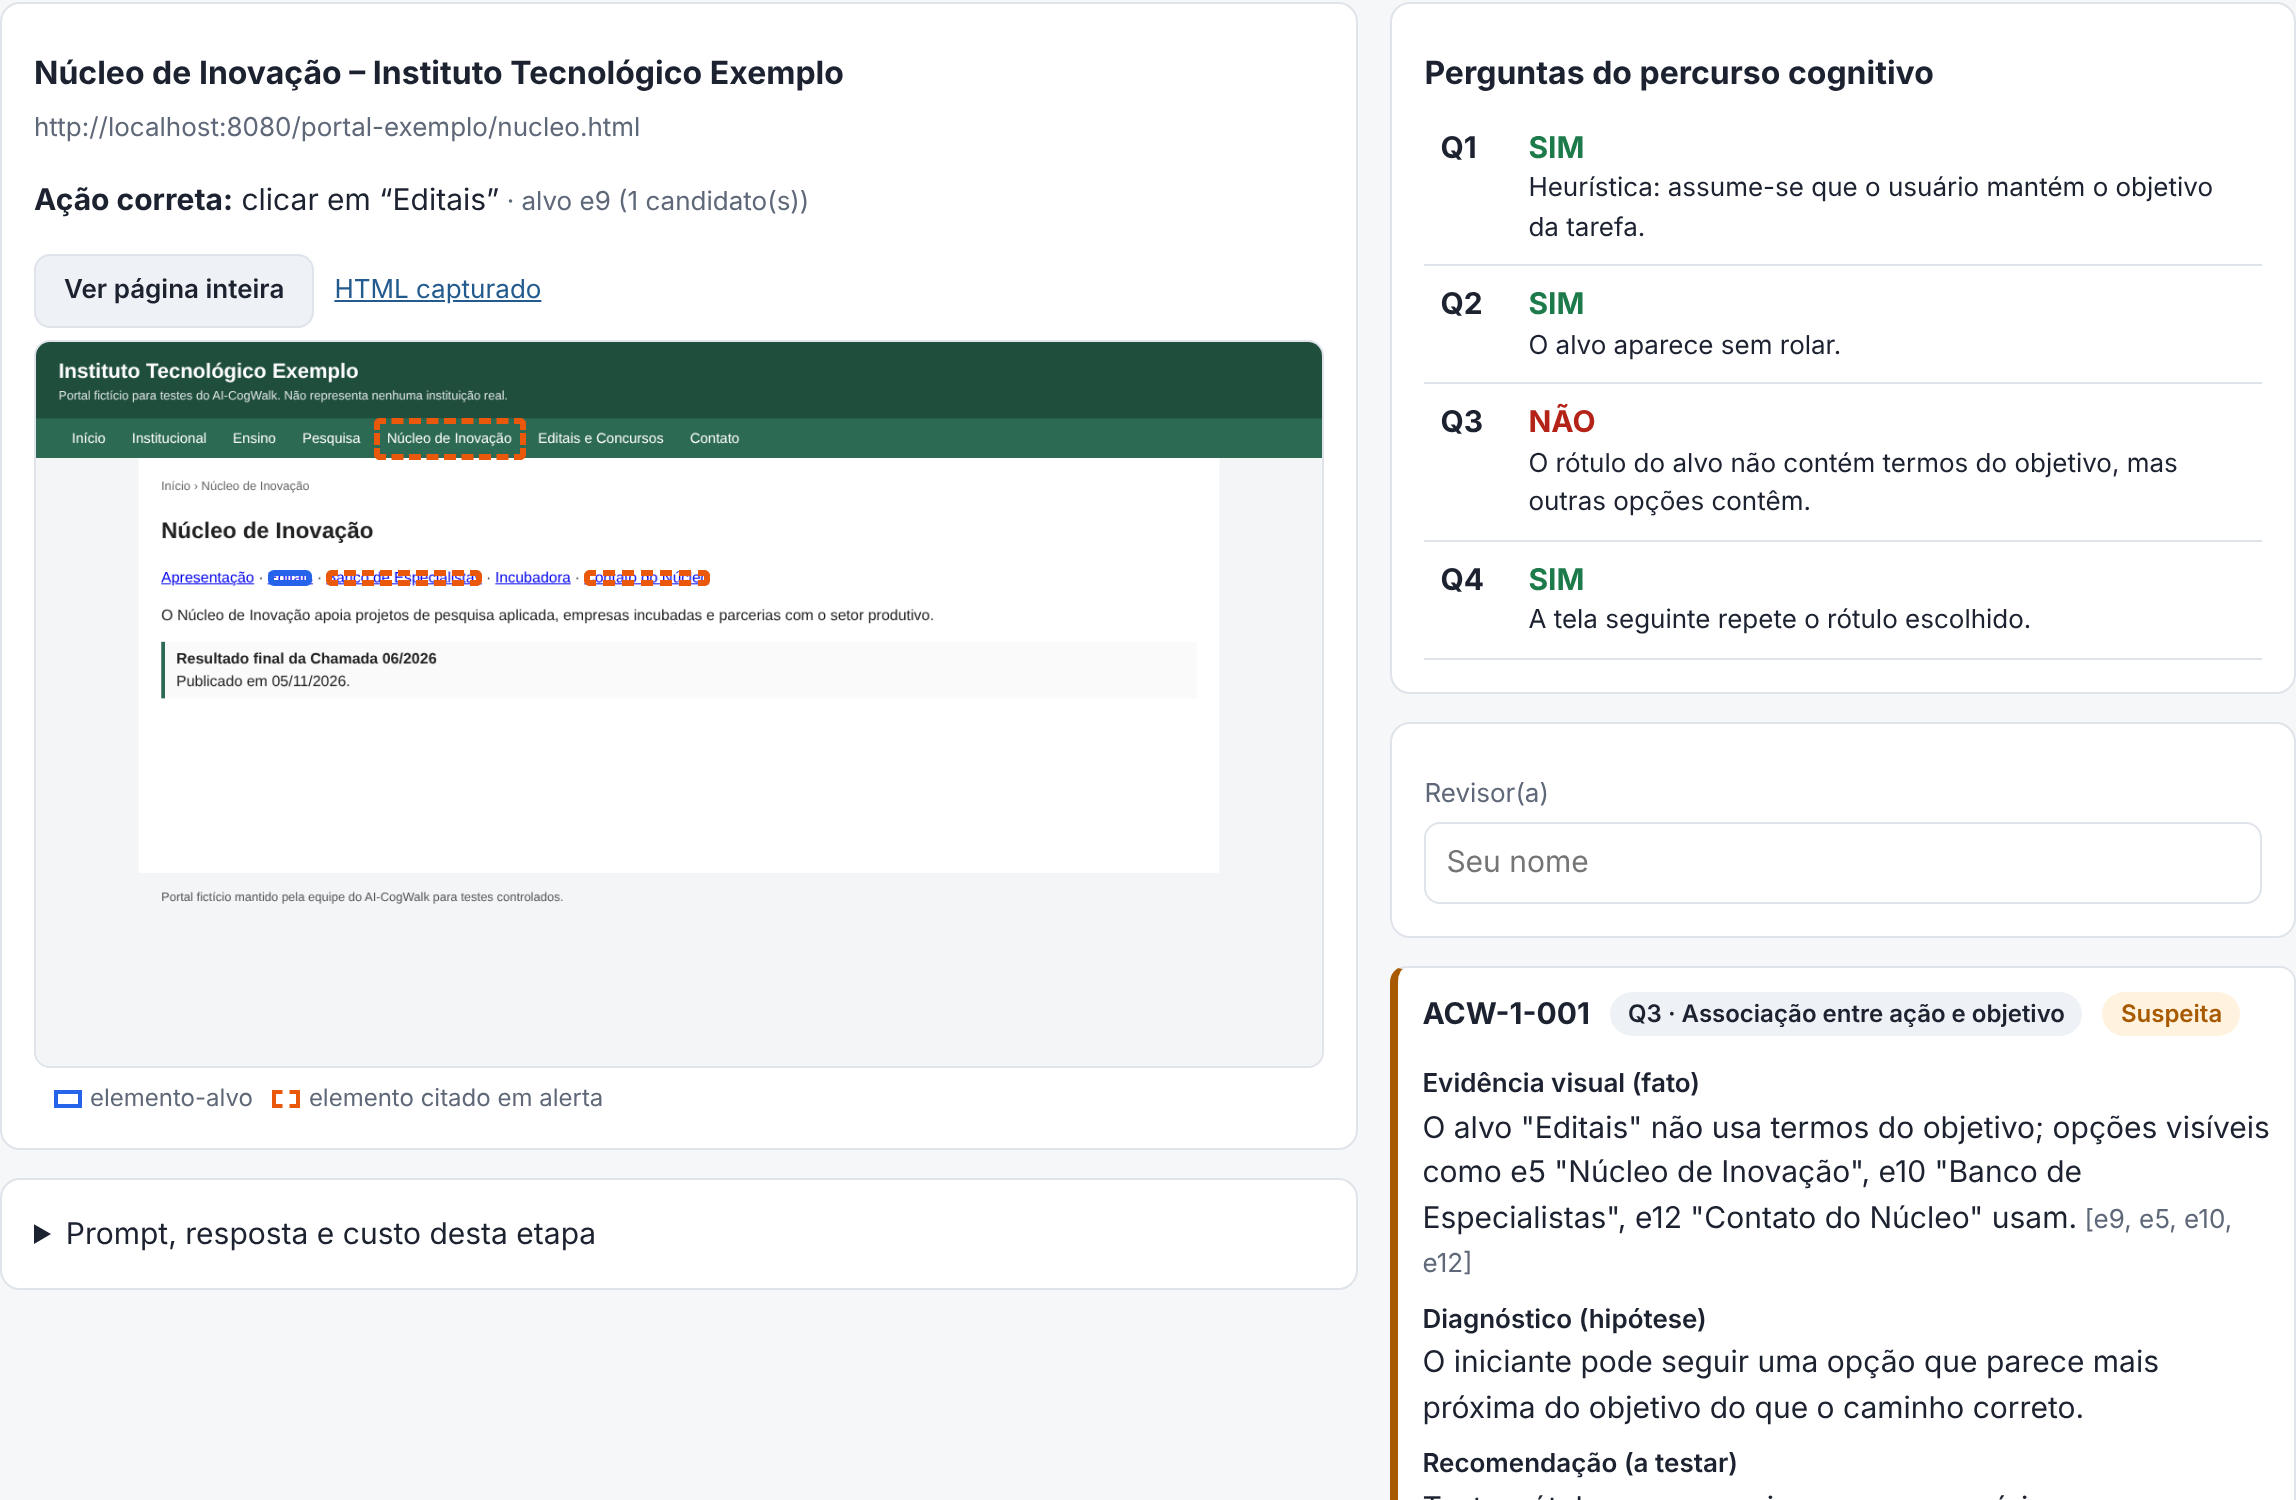
\includegraphics[width=\linewidth]{figuras/mvp-execucao.png}
\caption{Tela de revisão do protótipo (portal fictício, etapa 2, avaliador \textit{offline}). À esquerda, a captura com o elemento-alvo (contorno contínuo) e os elementos citados no alerta (contorno tracejado); à direita, as respostas a Q1--Q4 e o alerta, com evidência visual, diagnóstico e recomendação separados.}
\label{fig:mvp}
\end{figure}

\textbf{O que ainda não foi feito.} Nenhuma execução com o modelo multimodal foi feita até aqui, porque a chave de acesso à API ainda não foi configurada no ambiente. Também não há dados com participantes, que dependem de aprovação ética, e a calibração da confiança depende desses dados. O banco de casos humanos usado no \textit{few-shot} é provisório e ilustrativo, escrito apenas para testar o fluxo, e será substituído por casos observados antes de qualquer resultado. Os próximos passos técnicos são executar o caso piloto a partir de uma rede com acesso ao portal e as primeiras avaliações com o modelo nas condições C1 e C2.

%%%%%%%%%%%%%%%%%%%%%%%%%%%%%%%%%%%%%%
\section{Desenho Experimental}
\label{sec:experimento}

\textbf{Questões de pesquisa.} A questão central é: \textit{em que medida a incorporação de padrões de dificuldades observadas em usuários reais melhora a precisão, a cobertura e a confiabilidade dos alertas gerados por agentes multimodais durante percursos cognitivos de interfaces web não utilizadas na calibração?} Ela se desdobra em quatro questões:
\begin{itemize}[noitemsep, topsep=3pt, leftmargin=1.5em]
  \item \textbf{QP1:} quais tipos de dificuldade de usuários iniciantes são identificados ou negligenciados por agentes multimodais durante percursos cognitivos?
  \item \textbf{QP2:} a inclusão de padrões de interação humana melhora a precisão, a cobertura e a calibração da confiança dos alertas em relação a um percurso cognitivo com contexto, mas sem evidência humana?
  \item \textbf{QP3:} como os resultados variam entre modelos, aplicações, tipos de tarefa e execuções repetidas?
  \item \textbf{QP4:} o ganho obtido compensa o custo computacional e humano adicional?
\end{itemize}

\textbf{Hipóteses.} A comparação principal é entre C3a e C2 no Protocolo G (Seção~\ref{sec:abordagem}), em aplicações não vistas. \textbf{H1} (principal): C3a tem F1 maior do que C2. \textbf{H2}: C3a tem \textit{recall} maior do que C2, isto é, deixa menos problemas observados sem identificação, sem perda de precisão maior do que uma margem fixada antes da coleta. \textbf{H3}: os alertas de C3a são mais bem calibrados do que os de C2 (menor \textit{Brier score}). Para o Protocolo A, a hipótese é exploratória: \textbf{H4}, na mesma aplicação, C3b tem \textit{recall} maior do que C3a. O custo não é tratado como hipótese, já que mais processamento sempre consome mais recursos, e sim como avaliação de custo-benefício (QP4): custo adicional, em \textit{tokens}, tempo e minutos de revisão humana, por problema observado a mais que C3a identifica em relação a C2. Todas as hipóteses podem ser rejeitadas, e o estudo foi desenhado para que a rejeição também seja informativa.

\textbf{Referência empírica e inspeção por especialistas.} O estudo tem dois grupos humanos com papéis diferentes. A \textit{referência empírica principal} vem dos participantes iniciantes: um problema só conta como \textit{observado} quando aparece no comportamento de pelo menos um participante durante a tarefa. Os especialistas (C0) não formam a referência; eles são um \textit{método comparativo}, avaliado contra a mesma referência que a IA. O diagnóstico de um especialista não é necessariamente um problema que algum participante experimentou. Problemas apontados por especialistas ou pela IA, mas não observados, formam um conjunto à parte, de \textit{problemas suspeitos}: podem ser reais e não ter se manifestado numa amostra pequena, ou podem ser falsos. Eles não entram como acerto nem como erro na análise principal e são analisados separadamente, numa análise de sensibilidade.

\textbf{Construção da referência.} Os participantes realizam as tarefas sem conhecer a interface, pensando em voz alta. São registrados ações, caminhos alternativos, retornos, pedidos de ajuda, erros e manifestações de dúvida. Dois avaliadores independentes identificam as ocorrências e as classificam por tarefa, etapa e pergunta do percurso cognitivo, e um terceiro resolve os desacordos; a concordância é reportada com o $\kappa$ de Cohen \cite{cohen1960kappa}. O resultado são problemas \textit{observados}, com o número de participantes afetados, e ocorrências \textit{insuficientemente documentadas}, que ficam fora da análise principal.

\textbf{Correspondência entre alertas e problemas.} Um alerta conta como acerto quando aponta a mesma tarefa, a mesma etapa e a mesma causa de um problema observado. Essa correspondência é julgada por dois avaliadores que não sabem de qual condição veio o alerta (C0, C1, C2 ou C3), com os alertas misturados e a formatação padronizada, para que o estilo do texto não revele a origem.

\textbf{Condições.} A Tabela~\ref{tab:condicoes} apresenta as condições. C2 é a \textit{baseline} decisiva: sem ela, o estudo poderia atribuir ao \proj\ um ganho que já decorre do uso do contexto. Uma ablação restrita retira de C3a, um por vez, a evidência humana e a verificação de evidências, para indicar de onde vem o ganho. O Avenir-UX \cite{tan2026avenirux} será executado como \textit{baseline} externa se a reprodução for viável no tempo previsto.

\begin{table}[!ht]
\centering
\caption{Condições experimentais.}
\label{tab:condicoes}
\footnotesize
\begin{tabularx}{\linewidth}{@{}>{\raggedright\arraybackslash}p{2.9cm} Y Y@{}}
\toprule
\textbf{Condição} & \textbf{Funcionamento} & \textbf{Papel no estudo} \\
\midrule
C0 -- Especialistas & Percurso cognitivo convencional, feito por especialistas & Método comparativo humano \\
C1 -- LLM sem histórico & Recebe a tarefa e uma tela isolada & \textit{Baseline} simples \\
C2 -- LLM com contexto & Recebe a sequência de navegação e avalia dificuldades & \textit{Baseline} forte, próxima a \cite{zhong2025syntheticcw} \\
C3a -- \proj, Protocolo G & Contexto + Q1--Q4 + padrões humanos de \textit{outras} aplicações + verificação & Intervenção principal (H1--H3) \\
C3b -- \proj, Protocolo A & C3a + rastros de poucos participantes da \textit{mesma} aplicação & Análise exploratória (H4) \\
\bottomrule
\end{tabularx}
\end{table}

\textbf{Estratégia de \textit{prompting}.} A estratégia de \textit{prompting} é tratada como variável do método, registrada em cada execução, e não como detalhe de implementação. Em C1, C2 e C3 o \textit{prompt}-base é o mesmo: papel de avaliador de usabilidade com o perfil do iniciante, as quatro perguntas do percurso cognitivo, regras que separam o fato visto na tela da hipótese sobre o usuário e saída em JSON com esquema fixo. Esse \textit{prompt}-base é \textit{zero-shot}, de modo que as condições difiram apenas no contexto fornecido (tela isolada, histórico, verificação). O uso de exemplos (\textit{few-shot}) \cite{brown2020fewshot} fica restrito a C3a, em que os exemplos são justamente os padrões humanos observados em \textit{outras} aplicações; casos da aplicação avaliada nunca entram como exemplo, para não vazar a resposta, e cada execução registra a versão do banco de exemplos e quais casos foram usados. Não se pede cadeia de raciocínio explícita no texto da resposta; o modelo justifica cada pergunta em uma frase. Como a escolha da estratégia altera o perfil de erros dos modelos, o estudo piloto inclui uma calibração restrita a C2, comparando \textit{zero-shot}, \textit{few-shot} e cadeia de raciocínio explícita \cite{wei2022cot} sobre as mesmas capturas, antes de congelar a configuração do experimento principal. Cada combinação é executada três vezes, e um alerta é considerado estável quando aparece em pelo menos duas das três execuções.

\textbf{Separação entre calibração e teste.} A Figura~\ref{fig:split} mostra a separação no Protocolo G. As aplicações de calibração são usadas só para extrair padrões e ajustar a confiança; as aplicações de teste, com seus participantes, nunca são vistas pelo sistema antes da avaliação. No Protocolo A, a aplicação é a mesma, mas os participantes cujos rastros alimentam o sistema são adicionais e não fazem parte da referência; por isso os resultados de C3b não são apresentados como avaliação em aplicação desconhecida, e são reportados em separado.

\begin{figure}[!ht]
\centering
\resizebox{0.95\linewidth}{!}{%
\begin{tikzpicture}[font=\small, node distance=0.5cm and 0.9cm,
  cal/.style={draw=green!50!black, fill=green!8, rounded corners=3pt, align=center, minimum height=1.1cm, text width=3.0cm},
  tst/.style={draw=orange!80!black, fill=orange!10, rounded corners=3pt, align=center, minimum height=1.1cm, text width=3.0cm},
  arr/.style={-{Stealth[length=2mm]}, gray!70!black, line width=0.7pt}]
  \node[cal] (piloto) {Piloto e aplicações de calibração};
  \node[cal, below=of piloto] (padroes) {Padrões de dificuldade e taxas de acerto};
  \node[draw=violet!70, fill=violet!6, rounded corners=3pt, align=center, minimum height=1.1cm, text width=2.4cm, right=of padroes] (motor) {Motor \proj};
  \node[tst, right=of motor] (alertas) {Alertas nas aplicações de teste};
  \node[tst, above=of alertas] (ref) {Referência humana de teste (participantes não vistos)};
  \node[draw=gray!70, fill=gray!8, rounded corners=3pt, align=center, text width=2.6cm, minimum height=1.1cm, right=0.9cm of alertas.north east, anchor=west, yshift=0.8cm] (metr) {Precisão, \textit{recall}, F1, estabilidade, custo};
  \draw[arr] (piloto) -- (padroes);
  \draw[arr] (padroes) -- (motor);
  \draw[arr] (motor) -- (alertas);
  \draw[arr] (alertas.east) -- (metr.west);
  \draw[arr] (ref.east) -- (metr.west);
  \draw[dashed, red!70, line width=0.8pt] (ref.west) -| node[pos=0.25, above, font=\scriptsize, red!70!black] {sem acesso} (motor.north);
  \node[red!70!black, font=\large\bfseries] at ($(motor.north)+(0,0.35)$) {$\times$};
\end{tikzpicture}}
\caption{Protocolo G: separação entre dados de calibração (verde) e de teste (laranja).}
\label{fig:split}
\end{figure}

\textbf{Planejamento amostral.} A Tabela~\ref{tab:escopo} resume o planejamento. Os números são uma estimativa inicial: com quatro aplicações e seis participantes por aplicação, cada referência teria poucos problemas observados, e o Protocolo A, se retirasse participantes dessa amostra, reduziria a referência a quatro pessoas. Por isso, (i) o Protocolo A usa participantes \textit{adicionais}, e só será executado se o recrutamento permitir; e (ii) o tamanho final será definido por um \textit{piloto} com uma aplicação de calibração e cerca de cinco participantes. O piloto estima quantos problemas uma aplicação produz e a probabilidade média de um participante encontrar cada problema; com essa probabilidade, o modelo de descoberta de problemas de \cite{nielsen1993model} indica quantos participantes são necessários por aplicação para observar a maior parte dos problemas, e o número esperado de problemas indica se a diferença mínima de interesse em F1 entre C2 e C3a é detectável. Se o piloto mostrar poucos problemas por aplicação, a prioridade será aumentar o número de aplicações de teste, e não o de participantes por aplicação, já que a generalização depende do número de interfaces.

\begin{table}[!ht]
\centering
\caption{Planejamento inicial, a revisar após o piloto.}
\label{tab:escopo}
\small
\begin{tabularx}{0.9\linewidth}{@{}l Y@{}}
\toprule
\textbf{Elemento} & \textbf{Proposta inicial} \\
\midrule
Piloto & 1 aplicação de calibração, cerca de 5 participantes \\
Aplicações & 1 a 2 de calibração e 4 de teste, de domínios diferentes \\
Tarefas & 3 por aplicação, com níveis distintos de complexidade \\
Participantes (Protocolo G) & pelo menos 6 por aplicação de teste; total definido após o piloto \\
Participantes (Protocolo A) & 2 adicionais por aplicação, se o recrutamento permitir \\
Especialistas (C0) & 3 \\
Modelos multimodais & 2: um comercial e um aberto executado localmente \\
Repetições por configuração & 3 a 5 \\
Unidade de análise & problema observado, definido por aplicação, tarefa, etapa e causa \\
\bottomrule
\end{tabularx}
\end{table}

\textbf{Calibração da confiança.} A confiança de um alerta é a probabilidade estimada de que ele corresponda a um problema observado. Ela é estimada por categoria de problema e pergunta do percurso cognitivo (Q1--Q4), a partir dos alertas das aplicações de calibração já comparados com sua referência. Como algumas categorias terão poucos exemplos, a taxa de cada categoria é combinada com a taxa global por meio de uma média ponderada com \textit{prior} Beta (encolhimento), de modo que uma categoria com poucos alertas fique próxima da média geral, e categorias com menos de um número mínimo de exemplos, fixado após o piloto, usam apenas a taxa global. A calibração é avaliada só nas aplicações de teste, com o \textit{Brier score}, curvas de confiabilidade e o erro de calibração esperado (ECE) com poucas faixas de confiança. Uma confiança de 80\% está bem calibrada se, entre os alertas com essa confiança, cerca de 80\% forem confirmados. Se o número de alertas não permitir estimar esses indicadores com precisão razoável, a confiança será reportada em três níveis (baixa, média e alta), e a análise verificará apenas se a taxa de confirmação cresce do nível baixo ao alto.

\textbf{Métricas.} A Tabela~\ref{tab:metricas} lista as métricas. O tempo de revisão importa: uma ferramenta com bom \textit{recall} pode ser pouco útil se produzir dezenas de alertas de baixa qualidade, e por isso os relatórios de cada condição serão revisados com o tempo cronometrado.

\begin{table}[!ht]
\centering
\caption{Métricas e questões de pesquisa associadas.}
\label{tab:metricas}
\footnotesize
\begin{tabularx}{\linewidth}{@{}l Y c@{}}
\toprule
\textbf{Métrica} & \textbf{Interpretação} & \textbf{QP} \\
\midrule
Precisão (validade) & Dos alertas, quantos correspondem a problemas observados? & QP2 \\
\textit{Recall} (completude) & Dos problemas observados, quantos foram identificados? & QP2 \\
F1 & Equilíbrio entre precisão e \textit{recall} (métrica principal) & QP2 \\
Calibração & \textit{Brier score}, curva de confiabilidade e ECE & QP2 \\
Cobertura por tipo & Quais categorias e perguntas (Q1--Q4) são identificadas ou perdidas & QP1 \\
Suspeitos não observados & Quantidade e natureza dos alertas sem correspondência na referência & QP1 \\
Concordância & $\kappa$ entre avaliadores na referência e na correspondência & --- \\
Estabilidade & Variação dos alertas entre execuções idênticas (Jaccard entre conjuntos) & QP3 \\
Custo-benefício & \textit{Tokens}, tempo e minutos de revisão por problema observado identificado & QP4 \\
\bottomrule
\end{tabularx}
\end{table}

\textbf{Plano de análise.} O plano será registrado antes da coleta principal (pré-registro), com a unidade de análise, as métricas e os testes abaixo. Um problema é considerado detectado por uma condição quando aparece na maioria das repetições daquela configuração; a variação entre repetições é analisada à parte, como estabilidade. A comparação principal, C3a contra C2, é pareada sobre os mesmos problemas: a detecção será comparada com o teste de McNemar \cite{mcnemar1947} e, se o volume de dados permitir, com regressão logística de efeitos mistos, com efeitos aleatórios para aplicação e tarefa. Como quatro aplicações são poucas para um \textit{bootstrap} agrupado por aplicação, os intervalos de confiança \cite{efron1993bootstrap} serão agrupados por tarefa, e os resultados também serão apresentados por aplicação, para que a variação entre interfaces fique visível. As comparações secundárias terão correção de Holm, e o relato privilegiará tamanhos de efeito e intervalos, e não só valores-$p$. O estudo segue as diretrizes de experimentação de \cite{wohlin2012experimentation}.

\textbf{Estudos auxiliares opcionais.} Se houver tempo antes da coleta com pessoas, dois estudos menores podem usar dados públicos, sem fazer parte da pesquisa principal. Com o Rico \cite{deka2017rico}, mede-se se o modelo identifica corretamente elementos e rótulos da tela, separando erros de percepção de erros de raciocínio. Com o GUIDE \cite{yang2026guide}, que tem 120 demonstrações de 54 iniciantes anotadas por comportamento, intenção e necessidade de ajuda, testa-se se o agente detecta confusão e necessidade de ajuda; como esses rótulos não são problemas classificados por Q1--Q4, seria preciso definir antes uma correspondência entre os dois esquemas.

%%%%%%%%%%%%%%%%%%%%%%%%%%%%%%%%%%%%%%
\section{Aspectos Éticos}
\label{sec:etica}

O estudo envolve participantes humanos, gravações de navegação e relatos de dificuldade. O projeto será submetido ao Comitê de Ética em Pesquisa competente antes de qualquer coleta, que decidirá sobre os procedimentos aplicáveis; a Resolução CNS nº 510/2016 \cite{cns2016res510}, que trata de pesquisas em Ciências Humanas e Sociais, é a referência principal, e o tratamento de dados pessoais seguirá a LGPD \cite{brasil2018lgpd}. O protocolo prevê: termo de consentimento livre e esclarecido, com direito de desistência; minimização de dados, com gravação apenas da tela e do áudio necessários; anonimização de nomes, rostos e dados que aparecerem na tela; armazenamento seguro, com acesso restrito; e nenhum envio de gravações identificáveis a provedores de IA. Para isso, os rastros que alimentam o agente serão transcritos e anonimizados antes de qualquer uso, e o modelo aberto executado localmente servirá de alternativa quando o dado não puder sair da instituição. As aplicações avaliadas usarão ambientes de teste ou contas fictícias, para que nenhum dado real de usuários das aplicações seja exposto.

%%%%%%%%%%%%%%%%%%%%%%%%%%%%%%%%%%%%%%
\section{Plano de Pesquisa}
\label{sec:plano}

O plano tem seis etapas.
\begin{enumerate}[noitemsep, topsep=3pt, leftmargin=1.5em]
  \item \textit{Revisão e consolidação da lacuna}: mapeamento sistemático \cite{kitchenham2007slr} sobre percursos cognitivos automatizados, agentes de interface, avaliação de usabilidade com LLMs e usuários sintéticos, priorizando CWGPT, \textit{Synthetic Cognitive Walkthrough}, GUIDE e Avenir-UX.
  \item \textit{Reprodução das baselines}: selecionar as aplicações e implementar C1 e C2, medindo o que já é identificado antes de propor melhorias; reproduzir o Avenir-UX se for viável. Os estudos com Rico e GUIDE são opcionais.
  \item \textit{Construção do corpus humano}: aprovação ética, piloto para definir o tamanho da amostra, pré-registro do plano de análise, definição das tarefas, recrutamento de participantes com diferentes graus de experiência digital, coleta e construção da referência com avaliadores independentes.
  \item \textit{Desenvolvimento do \proj}: implementação da estruturação por Q1--Q4, do uso controlado de evidências humanas, da verificação e da calibração da confiança.
  \item \textit{Experimentos comparativos}: comparação principal entre C2 e C3a no Protocolo G, com dois modelos e execuções repetidas; C0, C1, a ablação e o Protocolo A como análises secundárias.
  \item \textit{Artigos e dissertação}: um primeiro artigo empírico, comparando a capacidade de LLMs e de avaliadores humanos de identificar barreiras de aprendizagem (etapas 2 e 3); e o artigo principal, com a proposta e a avaliação do \proj. Os artefatos que puderem ser compartilhados serão publicados.
\end{enumerate}

A Figura~\ref{fig:cronograma} apresenta o cronograma previsto para 24 meses.

\begin{figure}[!ht]
\centering
\resizebox{0.9\linewidth}{!}{
\begin{ganttchart}[
  hgrid, vgrid={*2{draw=none}, dotted},
  x unit=0.32cm, y unit chart=0.55cm,
  bar/.append style={fill=blue!25, draw=blue!60, line width=0.7pt, rounded corners=1pt},
  milestone/.append style={fill=red!50, draw=red!60},
  bar label font=\small, title label font=\small,
  bar height=0.55
]{1}{24}
  \gantttitle{Trimestres (24 meses)}{24}\\
  \gantttitlelist{1,...,8}{3}\\
  \ganttbar{Disciplinas obrigatórias}{1}{12}\\
  \ganttbar{Revisão e consolidação da lacuna}{1}{6}\\
  \ganttbar{Reprodução das baselines}{4}{9}\\
  \ganttbar{Ética e piloto}{4}{8}\\
  \ganttbar{Coleta e referência humana}{8}{13}\\
  \ganttmilestone{Qualificação}{12}\\
  \ganttbar{Desenvolvimento do \proj}{10}{16}\\
  \ganttbar{Experimentos comparativos}{15}{19}\\
  \ganttbar{Análise e artigos}{14}{21}\\
  \ganttbar{Redação da dissertação}{18}{24}\\
  \ganttmilestone{Defesa}{24}
\end{ganttchart}}
\caption{Cronograma previsto.}
\label{fig:cronograma}
\end{figure}

%%%%%%%%%%%%%%%%%%%%%%%%%%%%%%%%%%%%%%
\section{Riscos e Ameaças à Validade}
\label{sec:ameacas}

A Tabela~\ref{tab:riscos} lista os principais riscos e como serão tratados.

\begin{table}[!ht]
\centering
\caption{Riscos e tratamento.}
\label{tab:riscos}
\footnotesize
\begin{tabularx}{\linewidth}{@{}>{\raggedright\arraybackslash}p{4.6cm} Y@{}}
\toprule
\textbf{Risco} & \textbf{Tratamento} \\
\midrule
O LLM identifica apenas problemas óbvios & \textit{Baselines} fortes (C2, Avenir-UX) e tarefas com níveis distintos de complexidade \\
A IA inventa dificuldades & Exigir evidência verificável e permitir o estado ``não confirmado'' \\
Evidências humanas contaminam a avaliação & Separar participantes, aplicações e versões de calibração e de teste \\
Participantes pouco representativos & Recrutar pessoas com diferentes graus de experiência digital e reportar o perfil \\
Modelos mudam durante o experimento & Registrar versões, parâmetros, \textit{prompts} e respostas; incluir um modelo aberto com versão fixa \\
Poucas interfaces & Declarar os limites de generalização; se o piloto permitir, priorizar mais aplicações de teste em vez de mais participantes por aplicação \\
Amostra pequena por aplicação & Piloto para estimar problemas por aplicação e participantes necessários; Protocolo A só com participantes adicionais \\
Confiança mal calibrada em categorias raras & Encolhimento para a taxa global; níveis ordinais se o número de alertas for pequeno \\
Escopo excessivo & Foco em C2 contra C3a; dois modelos; Rico, GUIDE e Avenir-UX como opcionais \\
Correspondência alerta--problema subjetiva & Dois avaliadores cegos à condição, com concordância medida \\
Especialistas tomados como verdade & Referência empírica vem dos participantes; especialistas são método comparativo \\
Efeito do avaliador na referência & Dois avaliadores independentes e um terceiro para desacordos \cite{hertzum2001evaluator} \\
\bottomrule
\end{tabularx}
\end{table}

Em termos de \textit{validade de construto}, ``problema de usabilidade'' depende de como a referência é construída; por isso a definição de problema observado e o protocolo de rotulagem serão fixados antes da coleta. Quanto à \textit{validade interna}, o autor do sistema também escreve os \textit{prompts}; a correspondência cega e o uso de aplicações não vistas reduzem esse viés. Quanto à \textit{validade externa}, quatro aplicações web e participantes de uma região não representam todas as interfaces e populações. Quanto à \textit{validade de conclusão}, o número de problemas por aplicação pode ser pequeno, o que será tratado com análise agrupada e com o relato dos tamanhos de efeito e intervalos, não só de valores-$p$.

%%%%%%%%%%%%%%%%%%%%%%%%%%%%%%%%%%%%%%
\section{Considerações Finais}
\label{sec:final}

Este projeto parte de uma observação simples: modelos que navegam corretamente não necessariamente compreendem as dificuldades humanas. O \proj\ propõe investigar essa limitação e tentar reduzi-la com um percurso cognitivo estruturado e com evidências de interação humana usadas de forma controlada, sem prometer que a IA substituirá avaliadores ou testes com usuários. O recorte é a detecção de barreiras de aprendizagem em interfaces web, com agentes multimodais e evidências humanas independentes.

A dissertação não depende de o \proj\ superar as \textit{baselines}. Mostrar de forma sistemática em quais situações agentes multimodais deixam de identificar dificuldades, e por quê, também é conhecimento científico relevante, e é o objeto do primeiro artigo previsto.

%%%%%%%%%%%%%%%%%%%%%%%%%%%%%%%%%%%%%%
\section*{Disponibilidade dos Artefatos}
{\small
Um protótipo inicial (MVP) já implementa a navegação controlada, a avaliação Q1--Q4 nas condições C1--C3, o registro de \textit{prompts}, versões e custos e a exportação de relatórios. O protótipo, os \textit{prompts}, as respostas dos modelos e o conjunto de dados anotado serão publicados em repositório público ao longo do projeto, na medida em que os termos de consentimento e a anonimização permitirem.
}

\section*{Uso de Inteligência Artificial}
{\small
Em conformidade com o Código de Conduta para Autores da SBC, declara-se que ferramentas de IA foram utilizadas como apoio. O \textit{Claude} (Anthropic) foi utilizado como apoio à revisão da literatura, à conferência das referências e à redação e organização deste texto. O conteúdo científico, a verificação das referências e as conclusões apresentadas são de responsabilidade exclusiva do autor.
}

\bibliographystyle{sbc}
\bibliography{references}

\end{document}
